\chapter{Fernlokalisierung mit Bluetooth}
\label{ch:phase3}
War die Infrastruktur von WLAN Access Points bisher gegeben und die Hardware somit unveränderlich, soll diese nun ausstauschbar beziehungsweise erweiterbar sein.
Dies erlaubt die Implementierung eines Bereichsortungssystems, welches nicht an die 802.11 Spezifikation gebunden ist.
Es soll eine Funkübetragungstechnik gewählt werden, die es den Tags erlaubt die in Abschnitt \ref{ch:Einleitung:sec:Anforderungen} maximal geforderten drei Jahre Akkulaufzeit zu erreichen.\\
Da mehrere Topologien für das Stationsnetzwerk denkbar sind, werden die Begriffe Basisstation und AP im Folgenden nicht mehr gleichgesetzt.
Eine Möglichkeit wäre, APs einzusetzen, die eine zweite Funkübetragungstechnik beherrschen, optional könnnte diese Fähigkeit etwa über einen USB-Port nachgerüstet werden.
Stattdessen kann die neu eingesetzte Technik auch von der bestehenden Infrastruktur getrennt und eine neue Infrastruktur aus Basisstationen aufgebaut werden.
Als Kompromiss der vorherigen Möglichkeiten können sich die neuen Basisstationen auch mittels LAN oder WLAN in die bestehende Infrastruktur einfügen. 
Dieser Kompromiss ist grundsätzlich zu bevorzugen, da die Komplexität geringer als bei zwei eigenständigen Netzen ist.

\section{nRF52832}
Der nRF52832 ist eine System-on-Chip Lösung von Nordic Semiconductor.
Er vereint eine 32-bit ARM Cortex-M4F CPU, 512kB RAM und einen 2,4GHz Transceiver, der Bluetooth 5 inklusive Low Energy und das proprietäre ANT Protokoll unterstützt \cite{nordic2017nrf}.\\
Für diese Arbeit wird ein Adafruit Feather nRF52 verwendet, der nRF52832 wird deshalb im Folgenden auf nRF52 abgekürzt.
Das Adafruit Feather nRF52 besitzt neben dem nRF52832 Spannungswandler für die 3,3 Volt Umwandlung und einen Schaltkreis für die Verwendung mit Lithium Akkus. Die verbaute CP2104 USB-to-Serial Schnittstelle erlaubt es, den Chip über USB zu programmieren.\\
Abb. \ref{fig:nrf52layout} zeigt das Adafruit Feather nRF52.
Auch Nordic Semiconductor gibt einige typische Stromverbräuche für ihr System-on-Chip an, diese sind in Abb. \ref{fig:nrf52consumption} aufgeführt.

\begin{figure}[h]
  \centering
	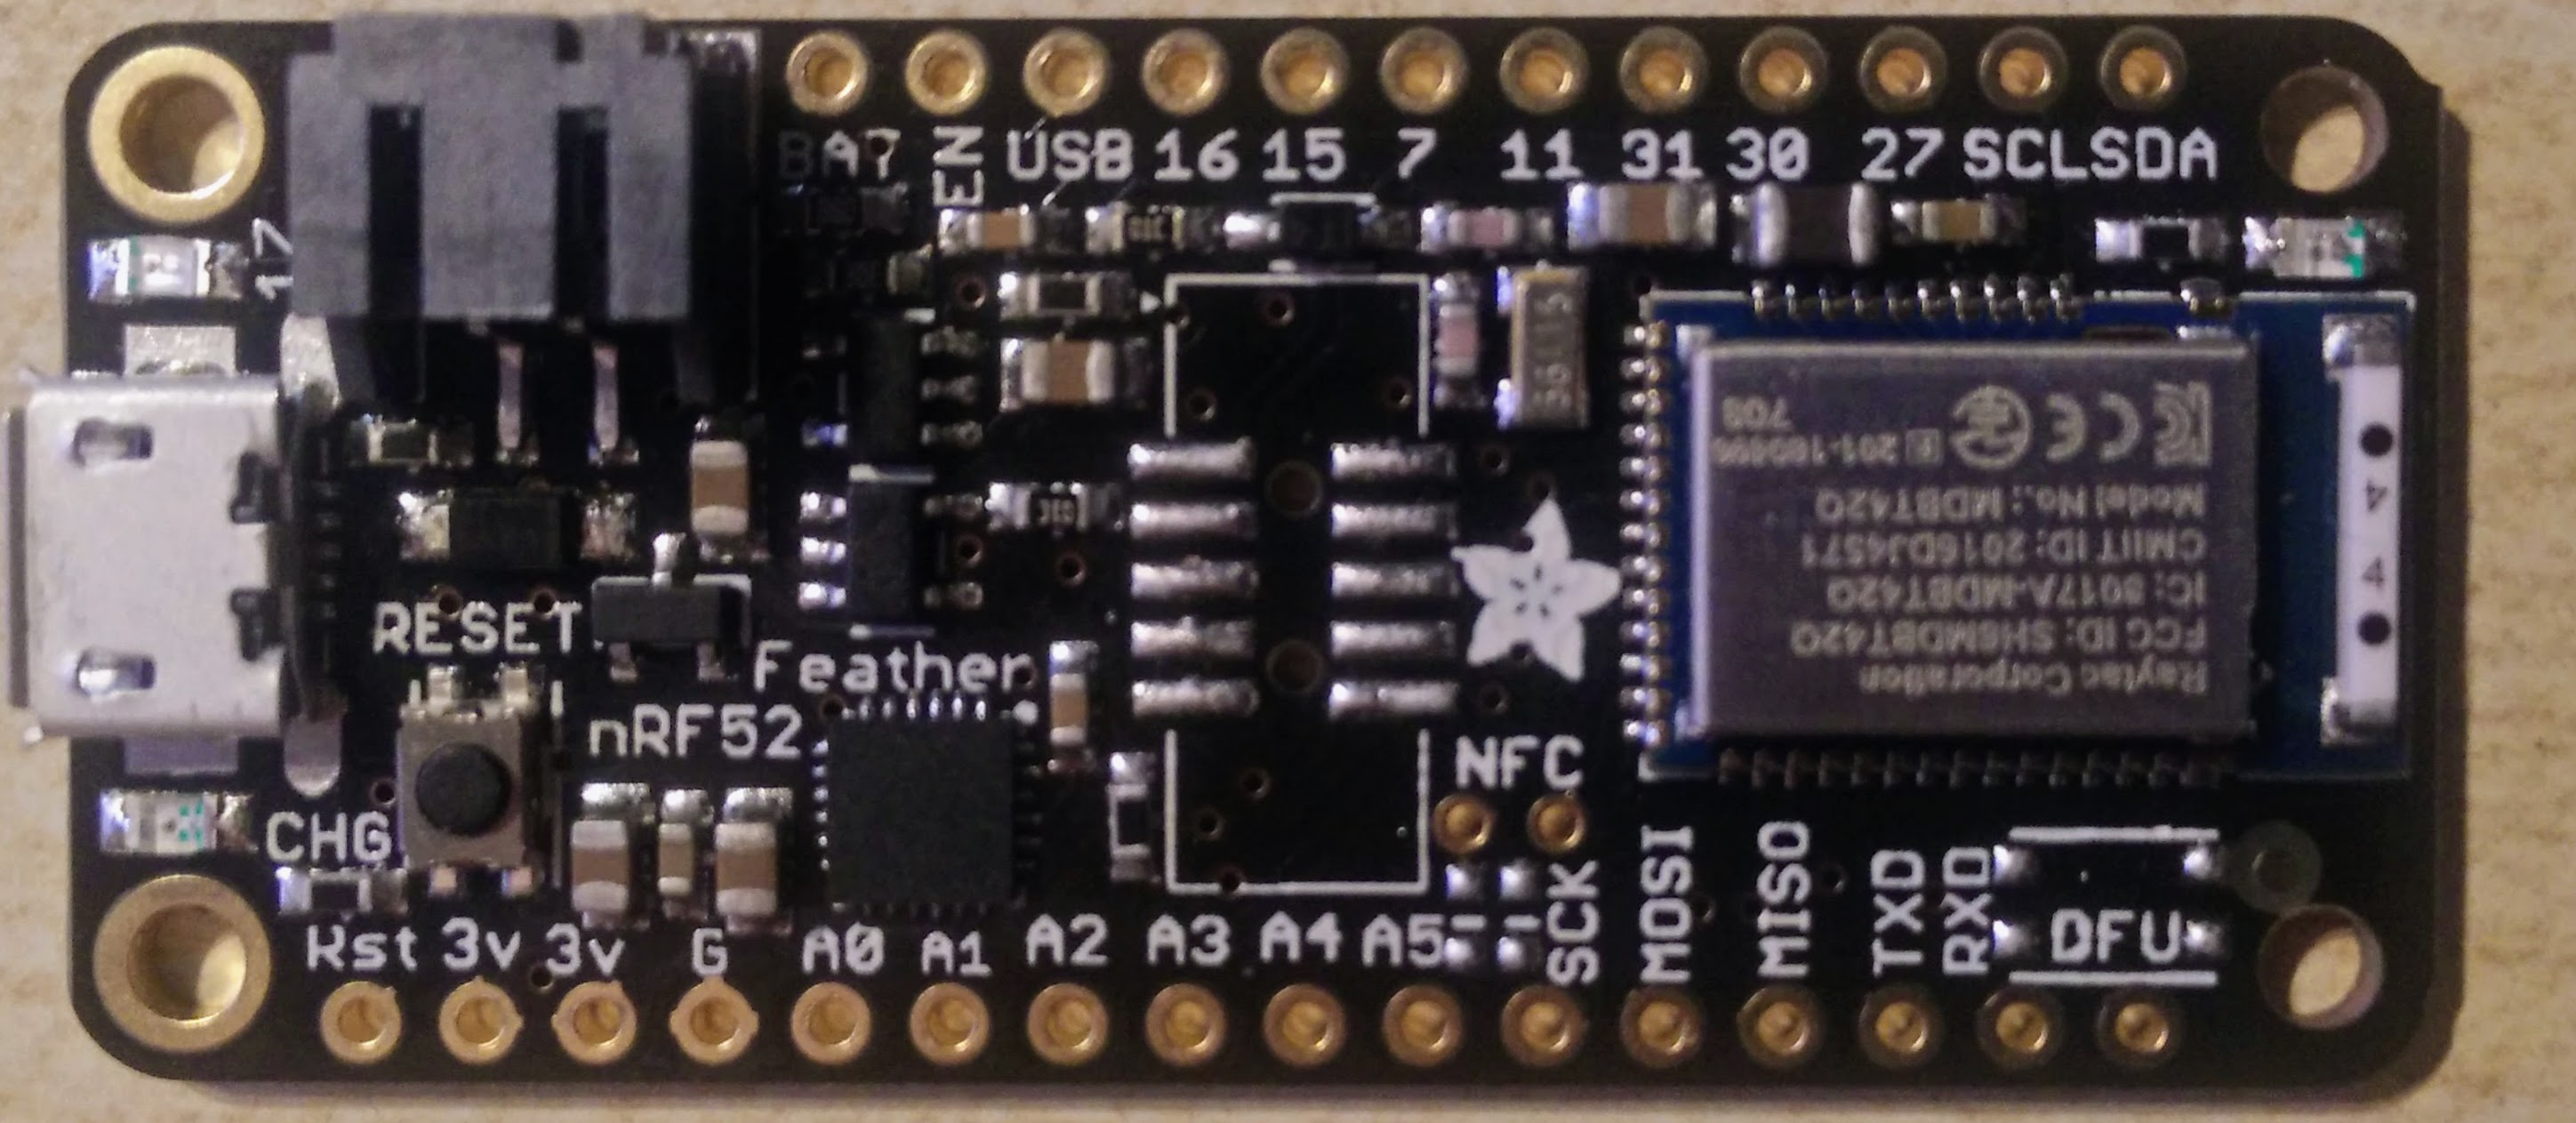
\includegraphics[width=\textwidth]{images/nrf52layout.jpg}
  \caption{Adafruit nRF52 Feather}
  \label{fig:nrf52layout}
\end{figure}

\begin{figure}[h]
  \centering
	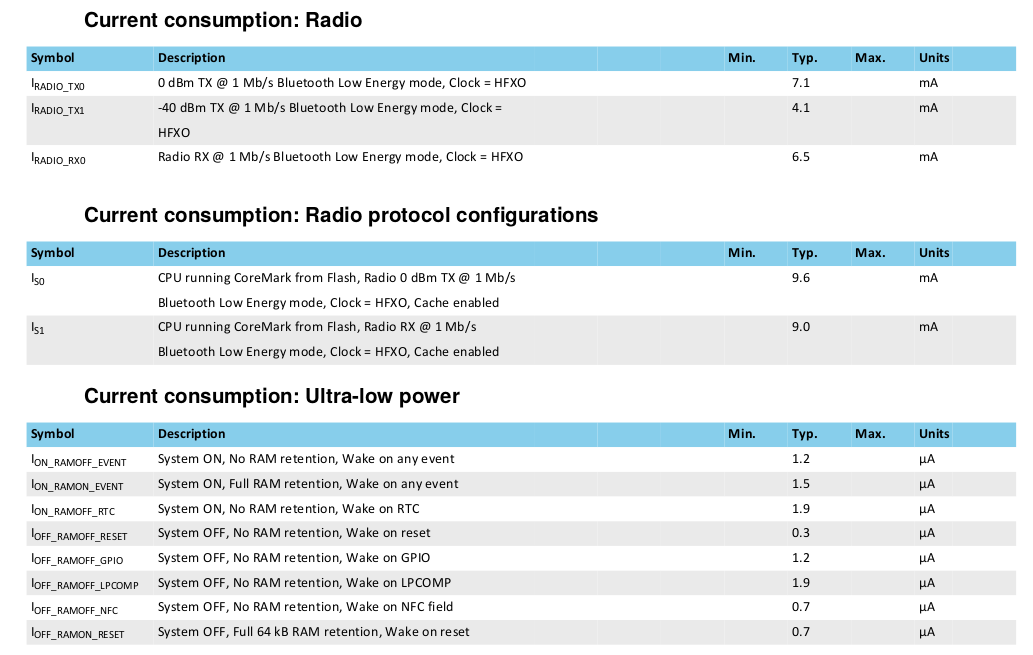
\includegraphics[width=\textwidth]{images/nrf52consumption.png}
  \caption{Energieverbrauch des nRF52832 in verschiedenen Zuständen, aus \cite{nordic2017nrf}}
  \label{fig:nrf52consumption}
\end{figure}


\subsection{Arduino Bluefruit nRF52 API}
Der nRF52 kann ebenfalls mit der Arduino IDE programmiert werden.\\
Dazu muss dieser zunächst das Board Support Package hinzugefügt werden \cite{fried2017nrf}.
In den Einstellungen wird unter \textit{Additional Boards Manager URLs} die URL \url{https://www.adafruit.com/package_adafruit_index.json} hinzugefügt.
Nach einem Neustart der Arduino IDE kann im \textit{Boards Manager} das Paket Adafruit nRF52 installiert werden.
Um das Board programmieren zu können wird zusätzlich das \textit{nrfutil} benötigt.
Dieses liegt nach der Installation der Boards in \\\texttt{~/.arduino15/packages/adafruit/hardware/nrf52/0.6.0/tools/nrfutil-0.5.2} und muss mit \texttt{sudo pip install -r requirements.txt} und \texttt{sudo python setup.py install} installiert werden.
Nachdem das Board in der IDE ausgewählt und über USB mit dem Computer verbunden wurde, kann nun eigener Code oder eines der Beispiele aus \textit{Examples for Adafruit Bluefruit nRF52 Feather} mit STRG+U auf den nRF52 geladen werden.\\
Es wird die Bluefruit nRF52 API Version 0.6.0 verwendet.

\section{BLE Advertising Implementierung}
\label{ch:phase3:sec:advertising}
Die Bluetooth Low Energy Implementierung ist an die Arbeit von Jianyong et al. angelehnt.
Es wird immer nach Ablauf des Sendeintervalls ein Advertising Paket gesendet.\\
In der Praxis wird dazu das Advertising Interval entsprechend gesetzt, dabei handelt es sich um einen in Bluetooth 4.0 spezifizierten Parameter für die Häufigkeit des Advertisings.
Da die Bluefruit nRF52 API keine Funktion zur Änderung dieses Wertes zur Verfügung stellt muss er direkt geändert werden.
Die entsprechende BLEAdvertising Klasse ist in \\\texttt{~/.arduino15/packages/adafruit/hardware/nrf52/0.6.0/libraries/}\\\texttt{Bluefruit52Lib/src} zu finden. \\
In \texttt{BLEAdvertising.cpp} ist \texttt{GAP\_ADV\_INTERVAL\_MS} auf 20 Millisekunden gesetzt, dieser Wert sollte erhöht werden, um den Energieverbrauch zu senken.
Beim nRF52 handelt es sich um ein Klasse 2 Bluetooth Gerät mit einer maximalen Sendeleistung bis 4 dBm.
Der ESP8266 erreicht bis zu 17 dBm, die maximale Reichweite sollte dementsprechend für den nRF52 geringer geschätzt werden.
Es wird eine Reichweite von 20 Metern angenommen und das Sendeintervall etsprechend der maximalen Bewegungsgeschwindigkeit von 30 km/h auf eine Sekunde gesetzt. 
In dieser Zeit kann sich ein Mitarbeiter maximal 9 Meter bewegen, es werden also bei der Durchquerung des Einflussbereichs mindestens drei Advertising Pakete vom Tag versendet.\\
Der Verbrauch sollte erneut mit dem Muker TM103 USB-Power-Meter gemessen werden.
Jedoch ist dieser nicht in der Lage den Stromverbrauch des nRF52 zu messen, da diese im niedrigen Mikroamper-Bereich liegen wenn nicht gesendet wird.
Die Sendeabschnitte sind zu kurz um einen messbaren Stromverbrauch zu erzeugen.\\
Deshalb soll zunächst Abb. \ref{fig:nrf52consumption} für eine theoretische Betrachtung des Verbrauchs herangezogen werden. 

\subsection{Theoretischer Verbrauch}
Für die Zeit in der nicht gesendet wird, wird der Zustand $I_{ON\_RAMOFF\_RTC}$ angenommen, da dieser den höchsten Verbrauch aufweist.
Für die Sendezeit wird $I_{RADIO\_TX0}$ angenommen, für ein Advertising Paket, welches zusätzlich den Gerätenamen "TestTag" versendet, werden 24 Bytes (192 Bit) gesendet.
Um die Kollisionsvermeidung einzufügen werden vorher 2000 Bit im Zustand $I_{RADIO\_RX0}$ empfangen, der die restliche Zeit wird in $I_{ON\_RAMOFF\_RTC}$ verbracht. 
Es müssen ebenfalls die weiteren Komponenten auf dem Feather bedacht werden. 
Adafruit gibt für den Spannungswandler einen Verbrauch von 55 Mikroamper und für den Lithium-Polymer-Ladeschaltkreis einen Verbrauch von bis zu 100 Mikroamper an \cite{fried2016lora}. 
Der Verbrauch des anderen Komponenten des Feather wird daher konservativ auf 155 Mikroamper geschätzt.\\[1cm]

$y = (1s-\frac{Bits_gesendet}{1000000 b/s} - \frac{Bits_empfangen}{1000000 b/s}) * (I_{ON\_RAMOFF\_RTC} + 155 {\mu}A) + \frac{Bits_gesendet}{1000000 b/s} * I_{RADIO\_RX0} + \frac{Bits_empfangen}{1000000 b/s} * I_{RADIO\_RX0}$\\[0.5cm]
$y = (1s - 0,000192s - 0,002s) * 0,1569mA + 0,000192 * 7,1mA + 0,002 * 6,5mA$\\[0.5cm]
$y \approx 0,156556mA + 0,001363mA + 0,013mA = 0,170919mA$ \\[1cm]

Wird erneut der 1400 mAh Lithium Polymer Akku angenommen beträgt die Laufzeit $1400mAh / 0,170919mA \approx 8191h$.
Dies entspräche circa 341 Tagen.\\
 

\subsection{Tatsächlicher Verbrauch}
Messungen zum Verbrauch ist in Abschnitt \ref{ch:realworld:sec:ble} zu finden. 

